\section{Mechanical design and locomotion system}
250 word + image

images/rover-front.png
images/rover-side.png
images/rover-top.png

\begin{figure}[htbp]
   \caption{\label{fig:rover} CAD view of the rover}
   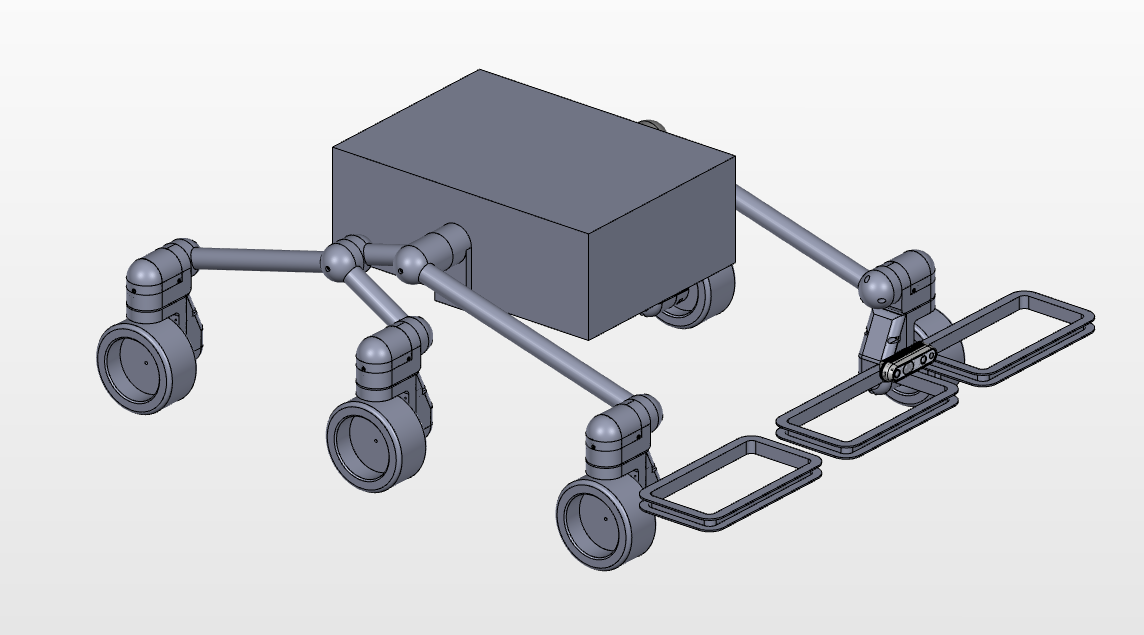
\includegraphics[width=\textwidth]{images/rover}
\end{figure}

\section{Sensors and landmine detection}
250 words

\section{Electronic circuit and control system}
250 words + image

\section{Area navigation}
250 words

\section{Mapping}

To map the competition area, our robot will use a custom localization system that we developped.
Similarly to GPS, our system computes the rover's position by using the \gls{rtt} of a radio signal to several fixed beacons, of which the position is known.

We use Decawave's DWM1000 radio modem with a custom protocol to measure the distance.
This gives us a good distance measurement accuracy: $1 \sigma = \SI{3}{\centi\meter}$.

Since we know the distance to each fixed beacons, as well as their positions, we can compute the position of the robot.
This is done using an \gls{ekf}, using the distance to a point as a correction function.
For the prediction step, we originally planned to use an inexpensive \gls{imu}, similar to the ones found in mobile phones.
However we probably won't implement it, due to time constraints.

The system was already tested on a \SI{20}{\meter} by \SI{20}{\meter} open field at our workshop.
We got very good positioning results and reliability, although we lacked time to do a quantitative analysis of the measurement accuracy and precision.
According to simulation, we should be within \SI{10}{\centi\meter} of ground truth.
As the reliability so far is good, we will be using this system only for Minesweepers 2018.


\section{Rough environment handling}

250 words

\textbf{YOUTUBE VIDEO}
